\subsection{Installation mit dem LiquidLauncher}

Für Windows und Linux gibt es den LiquidLauncher, der die Installation des Hacks deutlich vereinfachen sollte. Man findet diesen hier: \url{https://forum.ccbluex.net/thread.php?id=242}

Ich selber benutze aber kein Windows, sondern Linux und Mac, deswegen kann ich hierzu nicht wirklich was sagen.

\subsection{manuelle Installation}

\begin{hinweis}
    Wenn du schon mal Mods für Minecraft installierst hast (und zwar selber, nicht einfach nur ein fertiges Modpack starten!), lässt sich die Installation recht schnell zusammenfassen: LiquidBounce ist ein Mod.
\end{hinweis}

Die Vorgehensweise zur Installation ist bei den Versionen für Minecraft 1.8.9 und 1.12.2 gleich. Ich werde des Installationsvorgang aber nur für die Minecraft-Version 1.8.9 beschreiben.

Als erstes musst du im Minecraft-Launcher dir die Minecraft-Version 1.8.9 herunterladen. Dazu erstellst du dir über den Tab \textit{Profile} ein neues Profil und wählst als Version 1.8.9 aus. Dann startest du dieses Profil einmal, um es dann wieder zu schließen.

Als nächstes brauchst du Forge. Ich empfehle die Version 11.15.1902 \footnote{\url{http://files.minecraftforge.net/maven/net/minecraftforge/forge/1.8.9-11.15.1.1902-1.8.9/forge-1.8.9-11.15.1.1902-1.8.9-installer.jar}}. Für die 1.12 hab ich die Version 14.23.0.2491 \footnote{\url{http://files.minecraftforge.net/maven/net/minecraftforge/forge/1.12.2-14.23.0.2491/forge-1.12.2-14.23.0.2491-installer.jar}}. Eigentlich sollte auch jede andere Version von Forge gehen, aber die oben genannten funktionieren auf jeden Fall. Hast du den Forge-Installer heruntergeladen, musst du ihn nur noch ausführen und dich durchklicken. Der Installer lädt ein paar Dateien herunter und erstellt ein neues Profil im Minecraft-Launcher. Ist der Forge-Installer fertig, musst du den Minecraft-Launcher neu starten. Du solltest jetzt ein neues Profil mit dem Namen \textit{forge} haben.

Ich empfehle das neue Forge-Profil noch ein bisschen zu bearbeiten. Es bietet sich an, das Game-Directory bzw. Spiele-Verzeichnis auf \texttt{\%appdata\%/.minecraft/instances/liquidbounce1.8} zu ändern. Dann musst du im Minecraft-Verzeichnis noch einen Ordner mit dem Namen \texttt{instances} erstellen und in diesem dann einen Ordner \texttt{liquidbounce1.8}. Das hat den Vorteil, dass du mehrere Instanzen von Minecraft hast und problemlos zwischen den Versionen wechseln kannst.
Neben dem Game-Directory kannst du auch noch die Auflösung von Minecraft und die Java-Argumente einstellen. Mit dem Java-Argument \texttt{-Xmx4G} weist du Minecraft zum Beispiel 4GB RAM zu (um diese Einstellungen zu verändern, muss der Schieber bei \textit{Advanced Settings} auf an gestellt werden). Standardmäßig ist es nur 1GB, was oft Lags verursacht. Am besten so viel RAM wie möglich ist. Ein guter Richtwert ist die Hälfte des im PC verbauten RAMs.

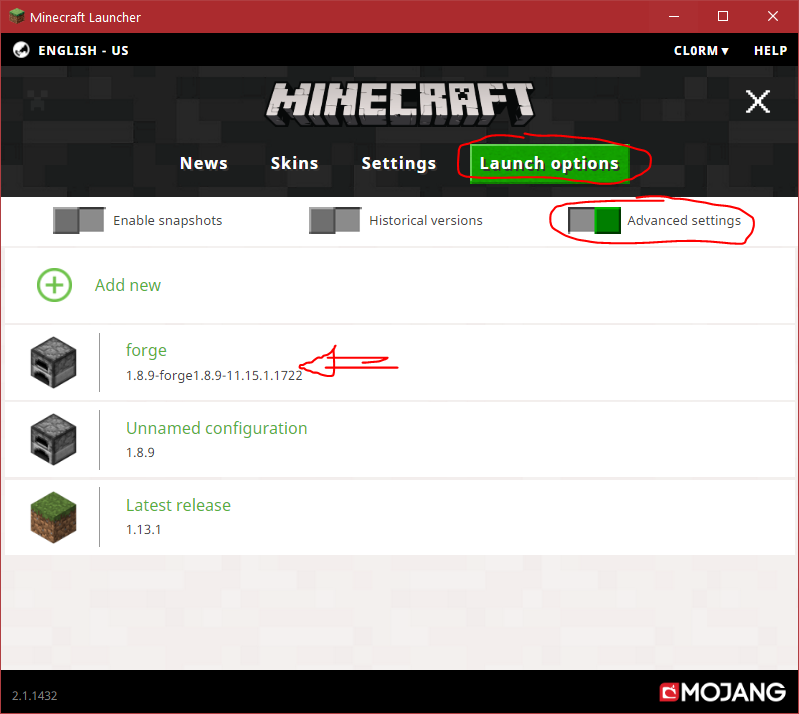
\includegraphics[scale=0.4, center]{TeX_files/pics/installation_1.png}

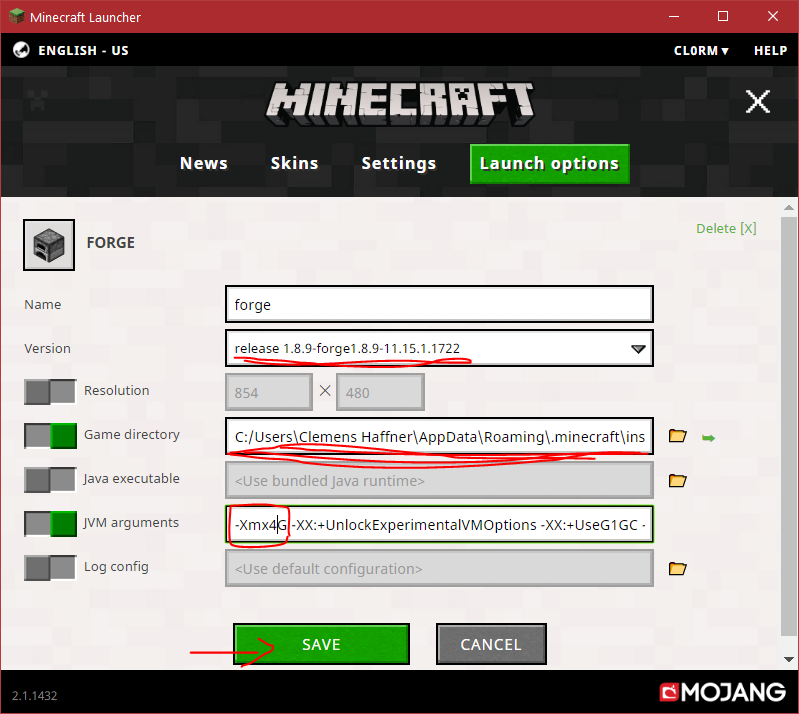
\includegraphics[scale=0.4, center]{TeX_files/pics/installation_advanced_settings.png}

Das Profil startest du einmal, damit Forge die Installation abschließen kann. Bist du im Minecraft-Mainmenu angekommen, kannst du Minecraft wieder schließen.

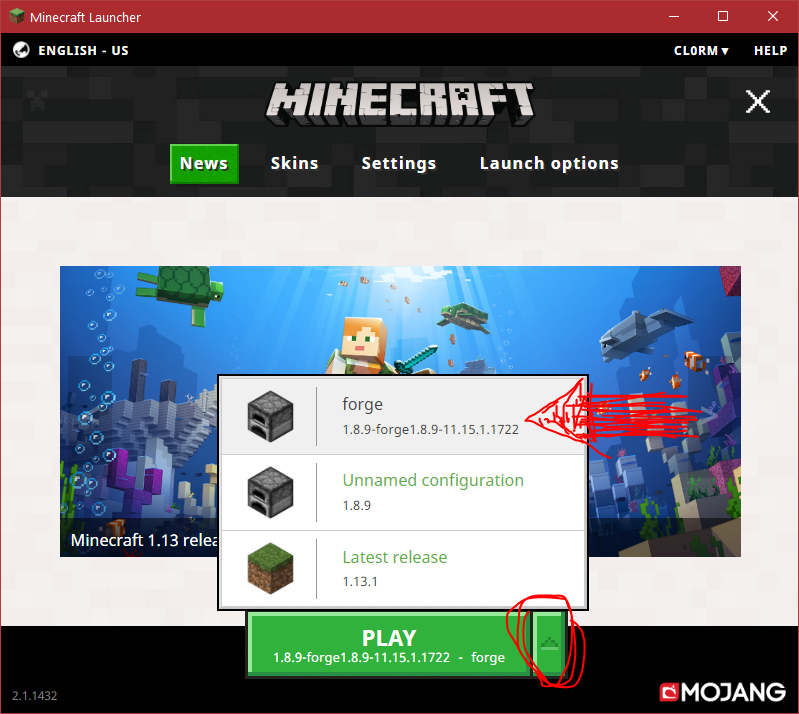
\includegraphics[scale=0.4, center]{TeX_files/pics/installation_starten.png}

Jetzt brauchst du den eigentlichen Hackclient. Dazu besuchst du \url{https://liquidbounce.net/} $\to$ Get Started $\to$ Minecraft-Version auswählen. Die heruntergeladene Datei kopierst du dann in \\ \texttt{\%appdata\%/.minecraft/instances/liquidbounce1.8/mods}